\startchapter{Preliminaries}
\label{Preliminaries}

This chapter briefly explains the key concepts used in this project.

\section{Multi-armed bandit \label{chap2:bandits}}

Multi-armed bandit is a problem setting where an agent makes a sequence of decisions in time $1, 2, ..., T$. At each time $t$ the agent is given a set of $K$ arms to choose and has to pull an arm. As a feedback for pulling an arm, it receives a reward for that arm, while the rewards of other arms cannot be determined. Problems represented as multi-armed bandits are stateless. They can be stochastic or adversarial. In a stochastic environment the reward of an arm is sampled from some unknown distribution, and in an adversarial setting the reward of an arm is picked by an adversary and is may be sampled from a distribution \cite{zhou2015survey}. In this project, we assume the problem setting as stochastic. \par

Personalized recommender systems recommend items (e.g., movies, news articles, web advertisements) to their users based on their predicted preference for these items. The feedback received from users response helps the system improve their prediction \cite{adomavicius2005toward}. However, to improve the quality of recommendations an item has to first be recommended. If an item is never recommended to users, the system cannot evaluate the feedback to improve it's quality of predictions on these items. Such problems where there is some information about the users which can be used to improve the quality of predictions without can be represented as a contextual bandit problem  \cite{vermorel2005multi}.

\section{Contextual Bandit \label{chap2:cb}}

In the theory of sequential decision-making, contextual bandit problems \cite{tewari2017ads} are placed between multi-armed bandit problems \cite{bubeck2012regret} and full-blown reinforcement learning (usually modeled using Markov decision processes with discounted or average reward to take optimal actions) \cite{sutton1998introduction}. Traditional bandit algorithms do not use any side-information or context. However, contextual bandit algorithms use context to learn and map contexts to appropriate actions. Since bandit algorithms only have a single state they do not have to consider the impact of their actions future states. Nevertheless, in many practical domains, such a problem setting is useful. This is true when the learner's action have limited impact on future contexts. In such a problem setting contextual bandit algorithms have shown great promise. Examples include web advertising \cite{abe1999learning} and personalized news article recommendation on web portals  \cite{li2010contextual,greenewald2017action}. \par

Formally a contextual bandit problem is a repeated interaction which takes place over $T$ rounds. At each round $t = 1,2,...T$ the environment reveals contexts $x_t \in X$ about the user and the available actions which are used by the learner to pick an action $a_t \in A$ which gives a reward $r_t$ revealed by the environment. The goal of the learner is to choose an action which would maximize cumulative reward $\sum_{t=1}^{T} r_t$. \par

We will now translate this problem setting for our adaptive teaching use case in which an algorithm $A$ which proceeds in discrete rounds $t = 1,2,3,...$. In round t: 
\begin{enumerate}
\item The algorithm observes the student context $x_s$ and a set $A_t$ of content items together with their feature vectors $x_{c}$ for $a \in A_t$. $X_{t}$ encapsulates $x_s$ and the context ${x_c}$ of all content items available in round $t$.
\item Based on observed rewards in previous rounds, $A$ chooses an arm $a_t \in A_t$. The arm $a_t$ is estimated to have the highest expected reward. In a stochastic setting, the expected reward is given as the inner product of an unknown arm-dependent parameter $\theta_{a,t}$ and the context $x_{t,a}$, that is, $E[r_{t,a}|\mathbf{x_{t,a}}] = x^{T}_{t,a}\mathbf{\theta_{t,a}}$. 
\item The student reveals the received reward $r_t$ for arm $a_t$ whose expectation depends on both the context $X_t$ and the arm $a_t$. 
\item The algorithm then improves it's content item selection strategy with the new observation $(x_t,a_t,r_t)$. It is important to emphasize here that no feedback namely, reward $r_{t}$ is observed for unchosen arms $a \neq a_t$ \cite{li2010contextual}.
\end{enumerate}

\section{Upper Confidence Bound (UCB) \label{chap2:UCB}}

An unavoidable challenge in bandit algorithms is to find the right balance between exploration and exploitation (Section \ref{chap1:useCase}). Upper Confidence Bound (UCB) comprises of a family of algorithms which try to find the best trade-off between exploration and exploitation. It is based on the principle of \textit{being optimistic} by choosing actions which have the highest potential for reward. The intuitive reason that this works is that when acting optimistically, one of two things happens. Either the optimism was well justified, in which case the learner is already acting optimally, or the optimism was not justified. In the latter case, the algorithm takes some action that they believed might give a reward when in fact it does not. If this happens sufficiently often, then the algorithm will learn the true reward of this action and not choose it in the future \cite{banditalgs}. UCB algorithms estimate the expected reward for each arm by adding estimated sample mean of an arm with it's upper confidence bound. \par

We will refer to Figure \ref{UCB} as an example to understand UCB. Let us assume we have three arms $a_1, a_2, a_3$. The reward distribution for each arm after several rounds is a Gaussian distribution $Q$ with mean $\mu$ and standard deviation $\sigma$. The y-axis is the probability of obtaining a certain reward for these arms. \par

\begin{figure}[h]
    \centering
    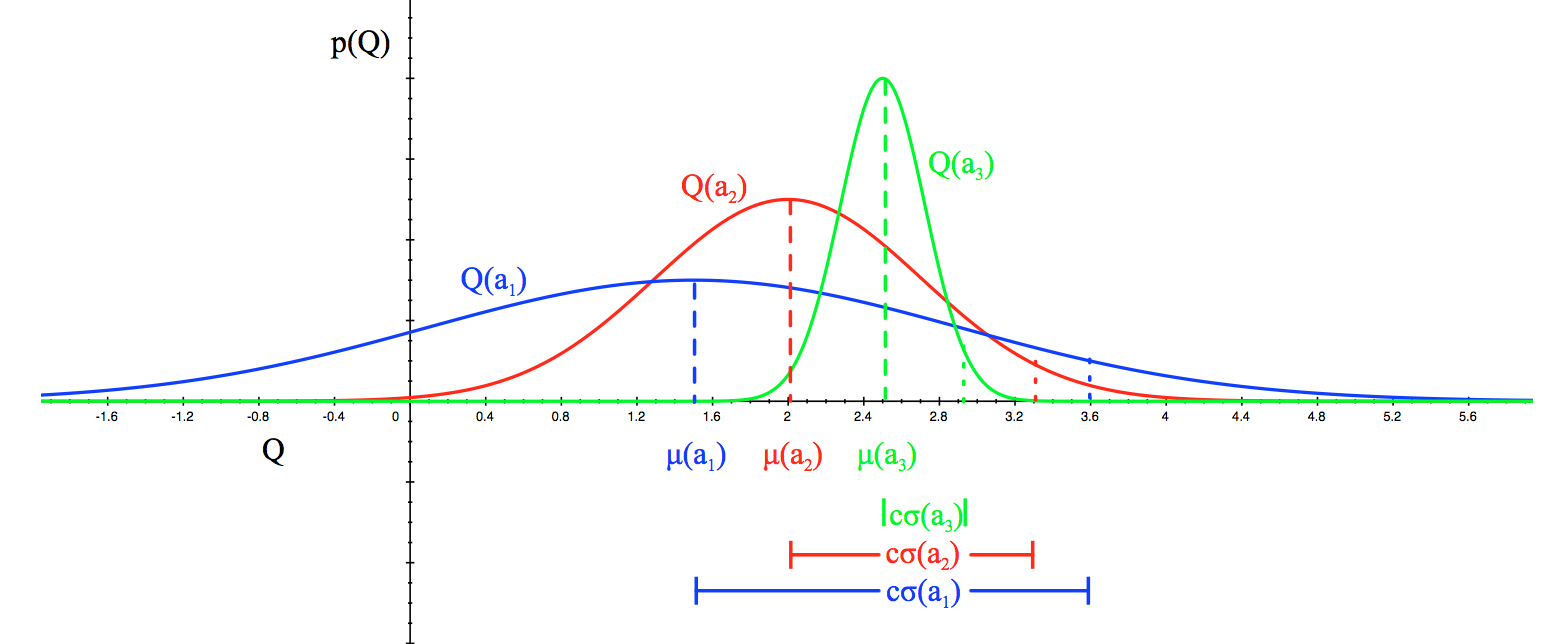
\includegraphics[scale=0.28]{Figures/UCB.png}
    \caption{An example: UCB}
    \cite{dsilver}
    \label{UCB}
\end{figure}

The upper confidence bound for each arm is given by $c\sigma(a_i)$. The distribution shows that the sum of the expected mean and upper confidence bound is highest for $a_1$. Hence the UCB algorithm will select $a_1$.
The reward received will reduce uncertainty around $a_1$. So for the next round, the algorithm once again finds the arm with the highest sum for the expected mean and upper confidence bound. This is repeated for $T$ rounds \cite{ankitmab}.

\section{Linear Upper Confidence Bound (LinUCB) \label{chap2:linUCB}}

LinUCB is a way to apply UCB to a more general contextual bandit setting where the UCB of each arm is computed efficiently by assuming the reward is linear, given as $E[r_{t,a}|\mathbf{x_{t,a}}] = x^{T}_{t,a}\mathbf{\theta_{t,a}}$. The estimated expected mean is parameterized over the context $x_{a}$ for each arm $a$. At round $t$ this is given as $\widehat{\theta}^{T}_{a}x_{t,a}$. The upper confidence bound around each arm $a$ at round $t$ is given as $\sqrt{x^{T}_{t,a}A^{-1}_{a}x_{t,a}}$. Here, $A_a$ is the co-variance over the context data $x_{t,a}$ for each arm $a$ at round $t$.  \par

LinUCB introduces a hyper-parameter $\alpha$, which allows us to control exploration over arms. This is achieved by scaling the upper confidence bound by $\alpha$. A higher value of $\alpha$ encourages exploration. As a result, the algorithm would need more rounds to explore before it begins exploiting. We can now compute \textbf{the expected estimated reward for an arm $a$ at round $t$ as $p_{t,a} = \widehat{\theta}^{T}_{a}x_{t,a} + {\alpha} \sqrt{x^{T}_{t,a}A^{-1}_{a}x_{t,a}}$}  \cite{li2010contextual}.\par